\documentclass[../../compsys.tex]{subfiles}
\begin{document}
\raggedbottom
\chapter{L13 — Internet Performance}
\vfill
\raggedbottom
\section{Properties of a Network Link}
\textit{Every physical link on the Internet is fully described by three fundamental parameters.}
\begin{enumerate}
  \item \textbf{Transmission rate} (\(R\)) — the maximum bit rate that can be carried while maintaining an acceptable error probability, measured in bit per second (e.g.\ 1 Gbps, 10 Gbps, 100 Gbps).
  \item \textbf{Length} (\(L\)) — the physical distance between the two end-points of the link, measured in metres.
  \item \textbf{Propagation speed} (\(v\)) — the speed at which a signal travels through the medium, measured in metre per second (\emph{$\approx$ the speed of light in fibre}).
\end{enumerate}
\newpage
\subsection{Packet Switches}
\textit{Packet switches interconnect links and move packets from their source toward their destination by consulting forwarding rules.}

\begin{center}
  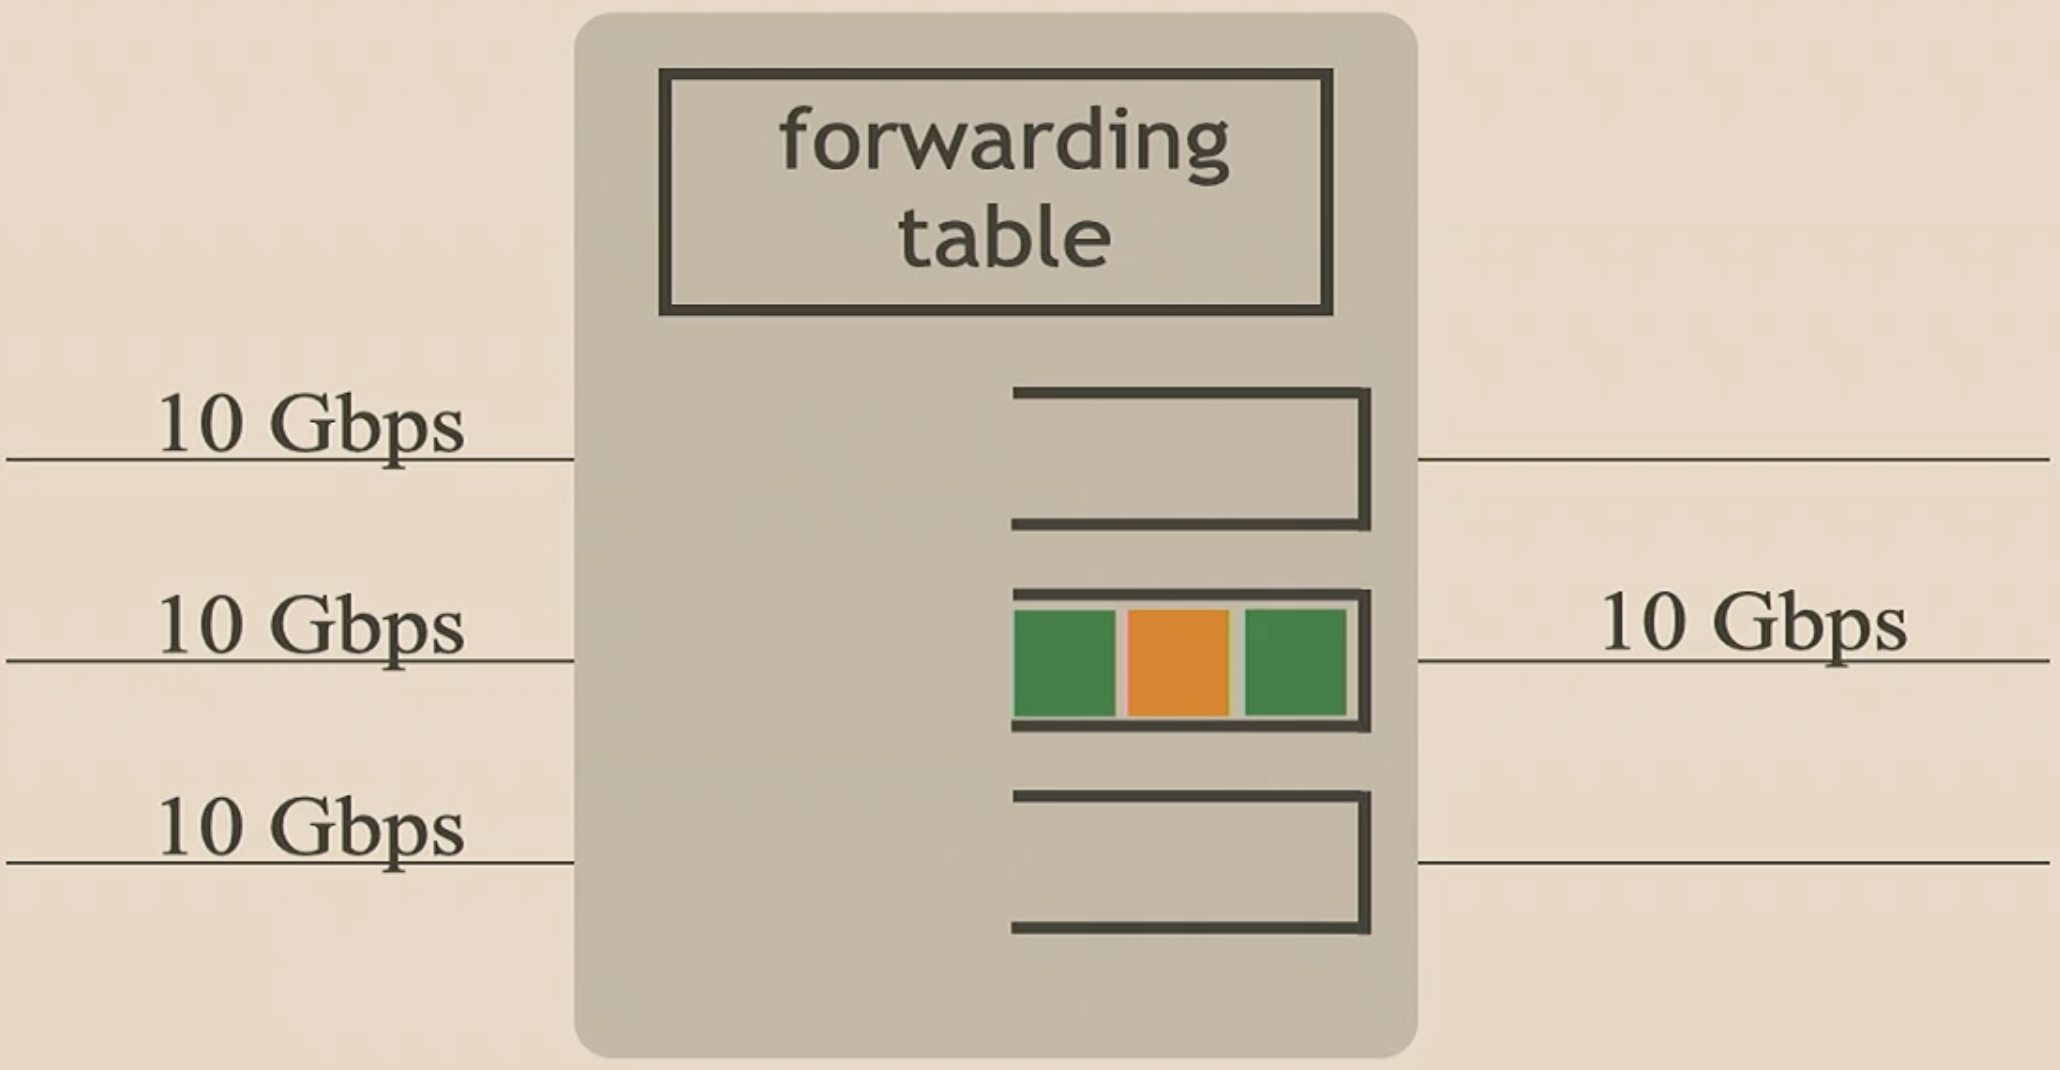
\includegraphics[width=.55\textwidth]{images/packet_switch.png}
\end{center}

A switch attaches to multiple (usually bidirectional) links.  
Packets arriving on any link are placed in a queue associated with the chosen outgoing link and are transmitted at that link's rate \(R\) (thus the queue drains at \(R\) whenever it is non-empty).

\subsubsection{Contents of a Packet Switch}
\textit{Inside a modern switch we find two essential data structures.}
\begin{enumerate}
  \item \textbf{Queues} — buffers that temporarily \emph{store} packets awaiting transmission.
  \item \textbf{Forwarding table} — metadata that maps header fields (e.g.\ destination address) to the appropriate outgoing link.
\end{enumerate}

\subsubsection{Store-and-Forward Packet Switching}
\textit{Most Internet switches use the store-and-forward paradigm.}
\begin{enumerate}
  \item The switch waits until \emph{all} bits of a packet arrive.
  \item It extracts the packet header and consults the forwarding table.
  \item It selects the best outgoing link and enqueues the packet.
  \item The packet is transmitted at the link's rate \(R\).
\end{enumerate}

\paragraph{Cut-Through Switching (for comparison).}  
Some high-performance switches begin forwarding as soon as the header has been received.  These are called \textbf{cut-through} switches; unless stated otherwise, assume switches in this course are store-and-forward.

\subsection{Network Congestion}
\textit{It is possible that a queue inside a packet switch fills up faster than it can drain.}

This can happen, for example, if we have a scenario where 3 × 10 Gbps links are all feeding traffic to a single 10 Gbps link. In this scenario, packets may arrive at a queue faster than they depart, which means that some packets may have to wait inside the queue and/or some packets may be dropped because they arrive at a moment when the queue is full.

This is an example of \textbf{network congestion}, which results in:
\begin{itemize}
  \item \textbf{Packet loss} — packets are dropped inside the network
  \item \textbf{Queuing delay} — packets have to wait in a queue
\end{itemize}

\section{Network Performance Analysis}
\textit{How do we reason about network performance, and what kind of performance does the Internet provide?}

\subsection{Basic Network Performance Metrics}
\textit{To quantify the performance of the network between a source and a destination, we use three simple metrics.}

\begin{enumerate}
  \item \textbf{Packet loss} — the fraction of packets from source to destination that are lost on the way
  \begin{itemize}
    \item[-] Measured in percentage, e.g., 1\% packet loss
  \end{itemize}
  
  \item \textbf{Packet delay} — the time it takes for a packet to get from source to destination
  \begin{itemize}
    \item[-] Measured in time units, e.g., 10 msec
  \end{itemize}
  
  \item \textbf{Average throughput} — the average rate at which the destination receives data
  \begin{itemize}
    \item[-] Measured in bits per second (bps)
    \item[-] Example: destination receives 1 GB of data in 1 min; average throughput = \(\frac{8 \times 10^9 \text{ bits}}{60 \text{ sec}} = 133.34 \times 10^6 \text{ bps} = 133.34 \text{ Mbps}\)
  \end{itemize}
\end{enumerate}

\subsection{Understanding Delay vs.\ Throughput}
\textit{To better understand the difference between delay and throughput, consider the following analogy.}

Visualize a path that is narrow and long: it fits only one person, and once a person gets on it, it takes 1 hour to traverse it. Suppose that there are multiple such paths between the same start and end points.

\subsubsection{Scenario 1: Small Group (3 Friends)}
Consider a group of 3 friends who want to go from start to end:
\begin{itemize}
  \item[-] \textbf{Option 1:} They all get onto the same path, one after the other
  \item[-] \textbf{Option 2:} Each friend gets on a different path and they traverse in parallel
\end{itemize}

Whether they pick option 1 or option 2, it takes about 1 hour for all of them to traverse. The choice of using parallel paths does not make a significant difference.

\subsubsection{Scenario 2: Large Group (1,000,000 People)}
Now consider a group of 1,000,000 people:
\begin{itemize}
  \item[-] \textbf{Option 1:} They all get on the same path, one after the other
  \item[-] \textbf{Option 2:} They use multiple paths in parallel
\end{itemize}

By using \(N\) parallel paths, they reduce the time it takes for all of them to traverse by about a factor of \(N\).

\paragraph{Key Insight.} The difference between the two scenarios is the amount of time that a person has to wait \emph{before} they get on the path:
\begin{itemize}
  \item In the 3-people scenario, the 2nd and 3rd person wait only a few extra seconds
  \item In the 1,000,000-people scenario, many people have to wait significantly longer
\end{itemize}

\paragraph{What Metric Do We Improve?}
Using parallel paths:
\begin{itemize}
  \item Does \textbf{not} improve the delay for one person to go from start to end
  \item \textbf{Does} improve the throughput: the rate at which people reach the end
\end{itemize}

\subsubsection{Application to Computer Networks}
\begin{itemize}
  \item \textbf{Packet delay} matters for exchanging small messages fast (e.g., interactive applications like voice or gaming)
  \item \textbf{Average throughput} matters for bulk transfers (e.g., downloading large files)
  \item They are related to each other, but not in an obvious way
\end{itemize}

\section{Packet Delay Components}
\textit{Estimating packet delay between various end-systems under different scenarios is one of the main activities of network engineers.}

\subsection{Direct Connection Scenario}
\textit{Two end-systems are directly connected through a single link.}

When the source transmits a packet over the link, there are two delay components:

\subsubsection{Transmission Delay}
The time to push all bits of the packet onto the link:
\[
\text{Transmission delay} = \frac{\text{packet size}}{\text{link transmission rate}}
\]

\textbf{Example:} For a 3-bit packet on a 1 Gbps link:
\[
\text{Transmission delay} = \frac{3 \text{ bits}}{1 \times 10^9 \text{ bps}} = 3 \text{ nsec}
\]

\subsubsection{Propagation Delay}
The time for the last bit to reach the destination:
\[
\text{Propagation delay} = \frac{\text{link length}}{\text{link propagation speed}}
\]

\textbf{Example:} For a 1-meter link with speed of light propagation:
\[
\text{Propagation delay} = \frac{1 \text{ meter}}{3 \times 10^8 \text{ m/s}} = 3.34 \text{ nsec}
\]

\paragraph{Total Packet Delay.}
\[
\text{Total packet delay} = \text{transmission delay} + \text{propagation delay}
\]

\subsection{Store-and-Forward Switch Scenario}
\textit{Two end-systems connected through a store-and-forward packet switch.}

In this scenario, the packet delay includes additional components:
\begin{align}
\text{Packet delay} &= \text{transmission delay over 1st link} \\
&\quad + \text{propagation delay of 1st link} \\
&\quad + \text{queuing delay at switch} \\
&\quad + \text{processing delay at switch} \\
&\quad + \text{transmission delay over 2nd link} \\
&\quad + \text{propagation delay of 2nd link}
\end{align}

\subsection{Queuing Delay}
\textit{The most variable component of packet delay.}

Unlike transmission and propagation delays, queuing delay cannot be precisely calculated because it depends on other traffic arriving at the switch. However, if we have information about the other traffic (e.g., its arrival rate at the queue and how bursty it is), it is possible to compute statistical measures of the queuing delay.

\subsubsection{Queuing Delay Analysis}
\textit{With an infinite queue assumption, queuing delay characteristics.}

\begin{itemize}
  \item[-] Approaches infinity if arrival rate $> $ departure rate
  \item[-] Depends on burst size when arrival rate $\le $ departure rate
\end{itemize}

\begin{center}
  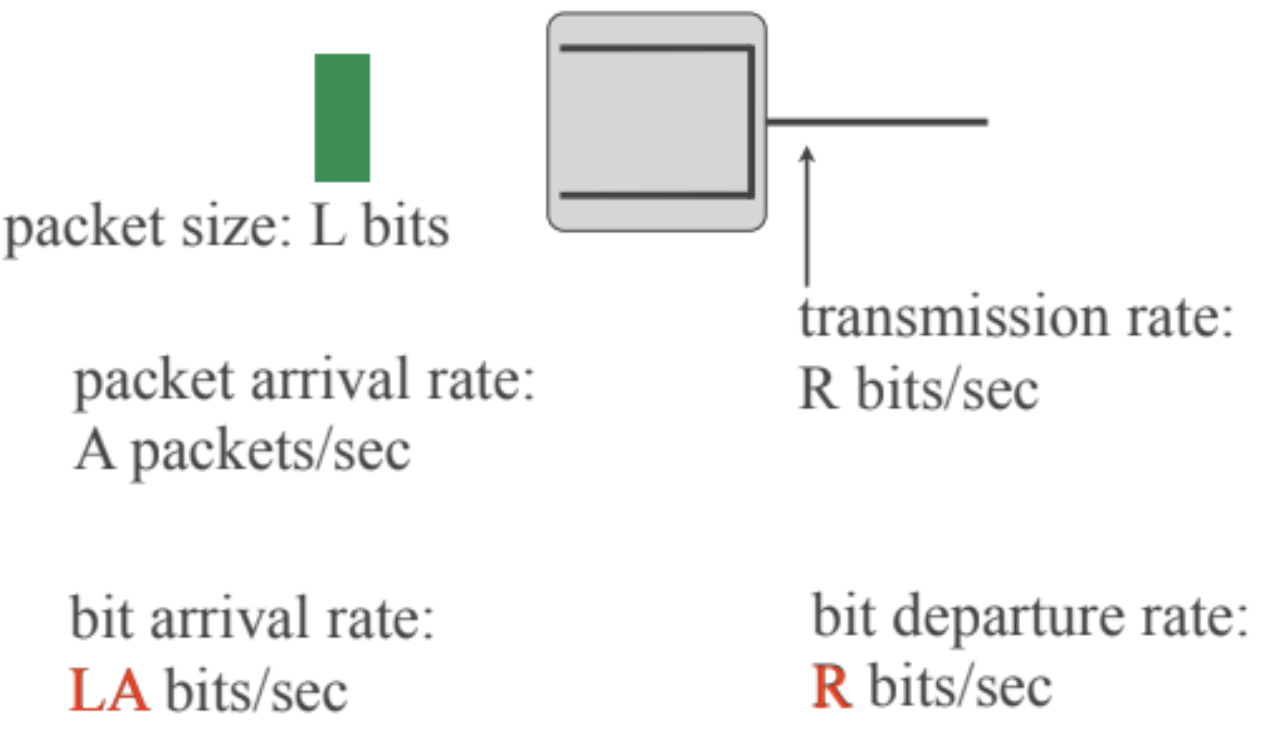
\includegraphics[width=.55\textwidth]{images/queuing_delay.png}
\end{center}

Consider a packet switch, with packets arriving and departing at an outgoing link at rate $R$. Suppose all packets have size $L$ bits and arrive at rate $A$ packets/sec (i.e., $LA$ bits/sec). Assuming an infinite buffer at the switch, we compare the bit arrival rate $LA$ to the bit departure rate $R$ to reason about queuing delay.

\begin{itemize}
  \item[-] \textbf{Scenario 1:} $LA > R$. Queuing delay grows without bound as more packets accumulate.
  \item[-] \textbf{Scenario 2:} $LA \le R$. Queuing delay depends on the burstiness of arrivals; instantaneous bursts can cause non-zero delay even if the average rate does not exceed $R$.
\end{itemize}

\begin{center}
  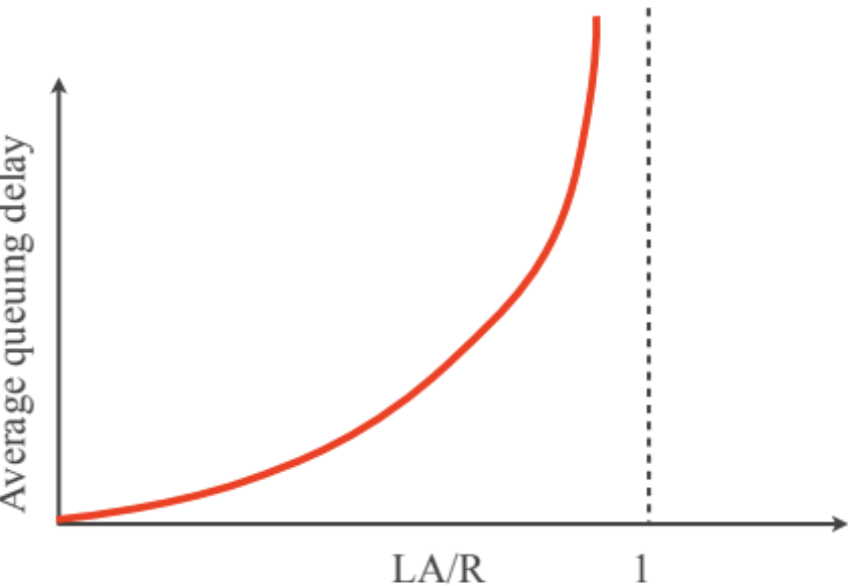
\includegraphics[width=.55\textwidth]{images/queuing_delay_plot.png}
\end{center}

This plot shows the average queuing delay experienced by a packet arriving at a queue, as a function of the arrival rate divided by the departure rate. As $LA/R$ approaches 1 (the arrival rate approaches the departure rate), the average queuing delay goes to infinity. The important characteristic of this curve is its exponential shape: there exists a threshold on the x-axis beyond which the curve increases rapidly. When a queue operates beyond this point, small changes in arrival rate can have a dramatic impact on queuing delay. In system design, queues should operate well below this threshold.

\subsubsection{Finite Queue Capacity}
\textit{Real switches have limited buffer capacity.}

\begin{center}
  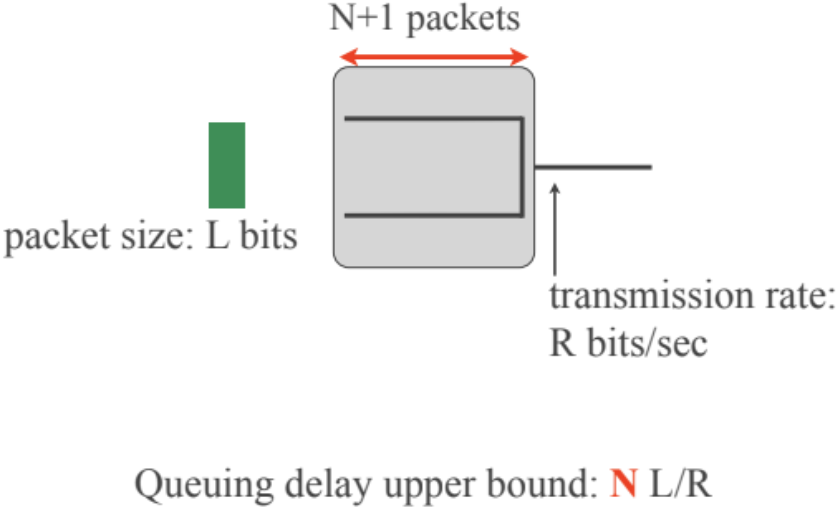
\includegraphics[width=.55\textwidth]{images/queuing_delay_upperbound.png}
\end{center}

In reality, switches don't have infinite queues. When a packet arrives and the queue is full, the switch drops the packet. The capacity of the queue imposes an upper bound on the queuing delay that a packet can suffer.

\paragraph{Maximum Queuing Delay.} If the queue can fit $N+1$ packets, what is the maximum queuing delay that a packet may experience? Assuming that processing delay is insignificant, the maximum queuing delay is $N$ times the transmission delay $(L/R)$. This occurs when a packet must wait for $N$ other packets to be transmitted over the outgoing link.
\newpage
\section{File Transfer Analysis}
\textit{Understanding delay and throughput for bulk data transfer.}

Packet delay between two end-systems has many components: transmission, propagation, queuing, and processing delays. The relative importance of each component depends on the network topology, link properties (transmission rates and propagation delays), switch operation, queue capacity, and traffic patterns.

\subsection{Direct Link File Transfer}
\textit{Two end-systems directly connected through a single link.}

Consider two end-systems connected by a physical link with rate $R$ bps. Previously, we computed the delay for one packet of size $L$ bits. Now we compute the delay for a file of size $F$ bits, assuming the source cuts the file into multiple packets of size $L$ bits and sends them consecutively.

\paragraph{Transfer Time Analysis.} The file transfer time consists of:
\begin{enumerate}
  \item The source pushes all $F$ bits onto the link: $F/R$
  \item The last bit propagates to the destination: propagation delay
\end{enumerate}

Total transfer time:
\[
\text{Transfer time} = \frac{F}{R} + \text{propagation delay}
\]

In practice, $F/R$ is typically large enough that the propagation delay becomes insignificant and can be ignored.

\paragraph{Average Throughput.} The source sent $F$ bits in approximately $F/R$ time units:
\[
\text{Average throughput} \approx \frac{F}{F/R} = R
\]

The throughput is always slightly smaller than $R$ due to the propagation delay. When two end-systems communicate over a link of transmission rate $R$, their throughput can never exceed $R$.

\subsection{Store-and-Forward with Multiple Links}
\textit{File transfer through packet switches.}

\begin{center}
  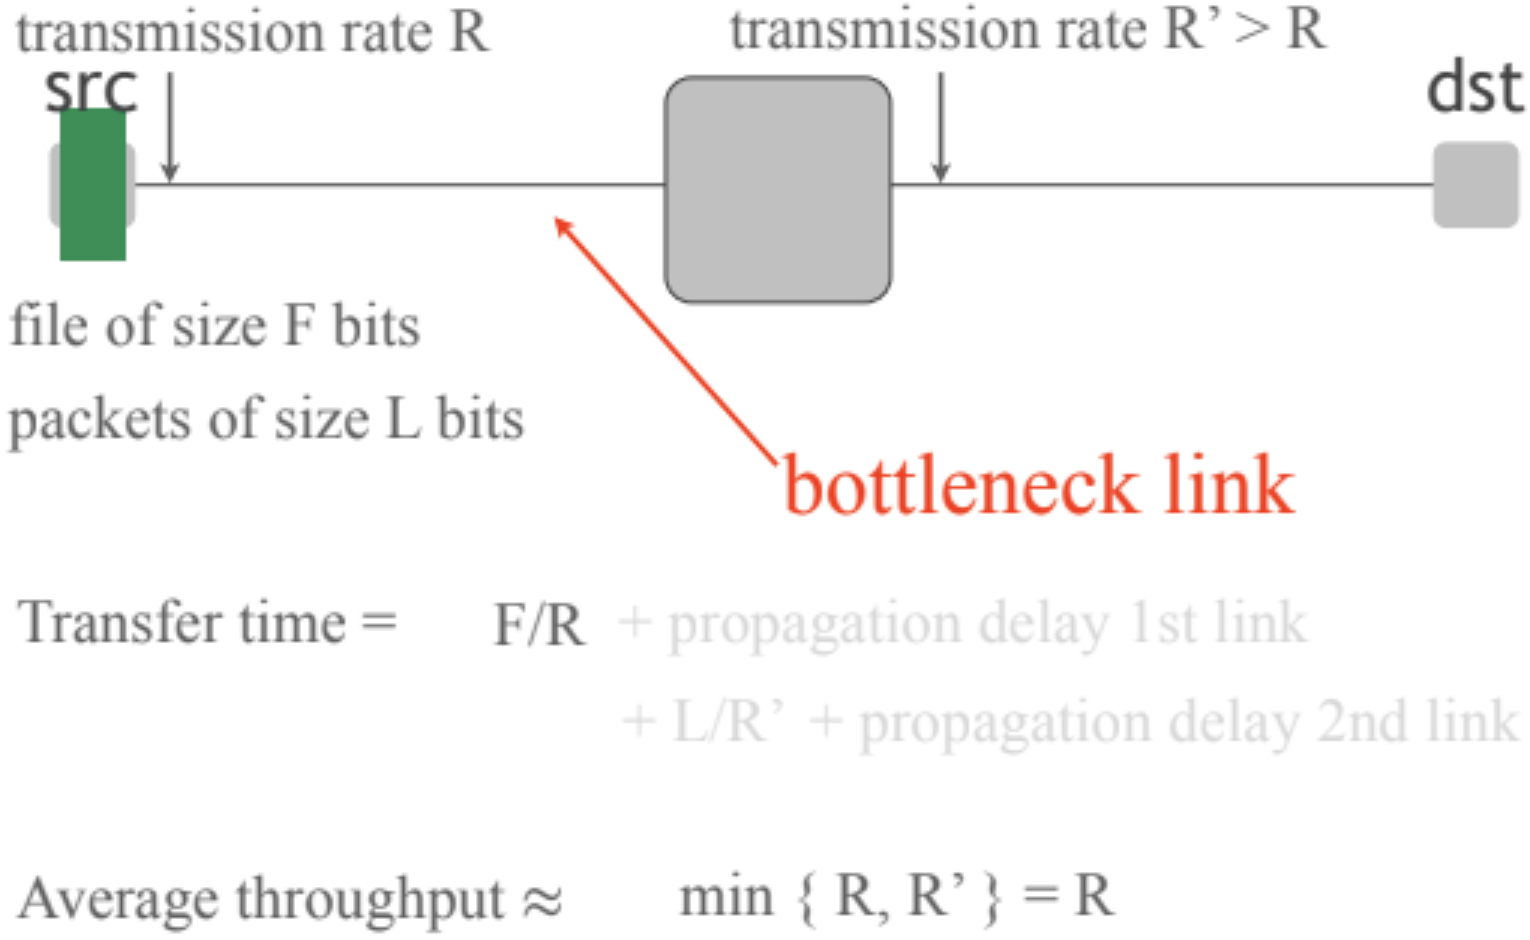
\includegraphics[width=.55\textwidth]{images/bottleneck_link.png}
\end{center}

Consider the same scenario with a store-and-forward packet switch between the end-systems. Assume the switch introduces negligible processing delay and receives no other traffic. Let the second link have transmission rate $R' > R$.

\paragraph{Transfer Time Analysis.} The transfer consists of:
\begin{enumerate}
  \item Source pushes all $F$ bits onto the first link: $F/R$
  \item Propagation delay of first link
  \item Last packet transmission on second link: $L/R'$
  \item Propagation delay of second link
\end{enumerate}

Since $R' > R$, packets leave the switch faster than they arrive, so the switch doesn't become a bottleneck. The total time is approximately $F/R$.

\paragraph{Bottleneck Link Concept.} When multiple switches are added between source and destination, the average throughput equals the transmission rate of the slowest link. This slowest link is called the \textbf{bottleneck link}, as it determines the maximum rate at which traffic can flow between the end-systems.

\subsection{Bottleneck Link Examples}
\textit{Concrete examples illustrating bottleneck behavior.}

\subsubsection{Example 1: Second Link as Bottleneck}
Consider a scenario where the first link has twice the transmission rate of the second link. If the first link supports 1 packet/sec for a given packet size, the second link supports 0.5 packet/sec.
\begin{center}
  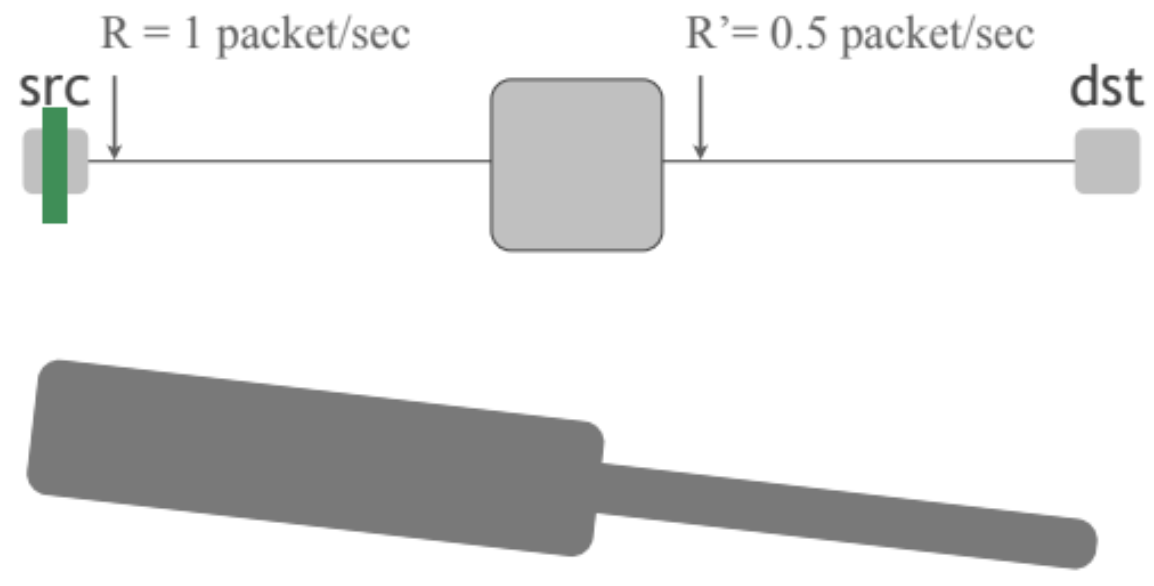
\includegraphics[width=.55\textwidth]{images/bottleneck_example1.png}
\end{center}
When the source transmits at 1 packet/sec, packets arrive at the switch faster than they can be transmitted on the second link. The switch must space them out, transmitting at only 0.5 packet/sec on the second link. This is analogous to a bottle where the narrow neck (second link) determines the flow rate, regardless of the bottle's capacity.

\subsubsection{Example 2: First Link as Bottleneck}
Now consider the reverse scenario where the second link has twice the transmission rate of the first link. If the source transmits at 0.5 packet/sec, the switch can immediately forward packets on the faster second link without spacing them out. However, it cannot bring packets closer together; it maintains the existing spacing determined by the first link.
\begin{center}
  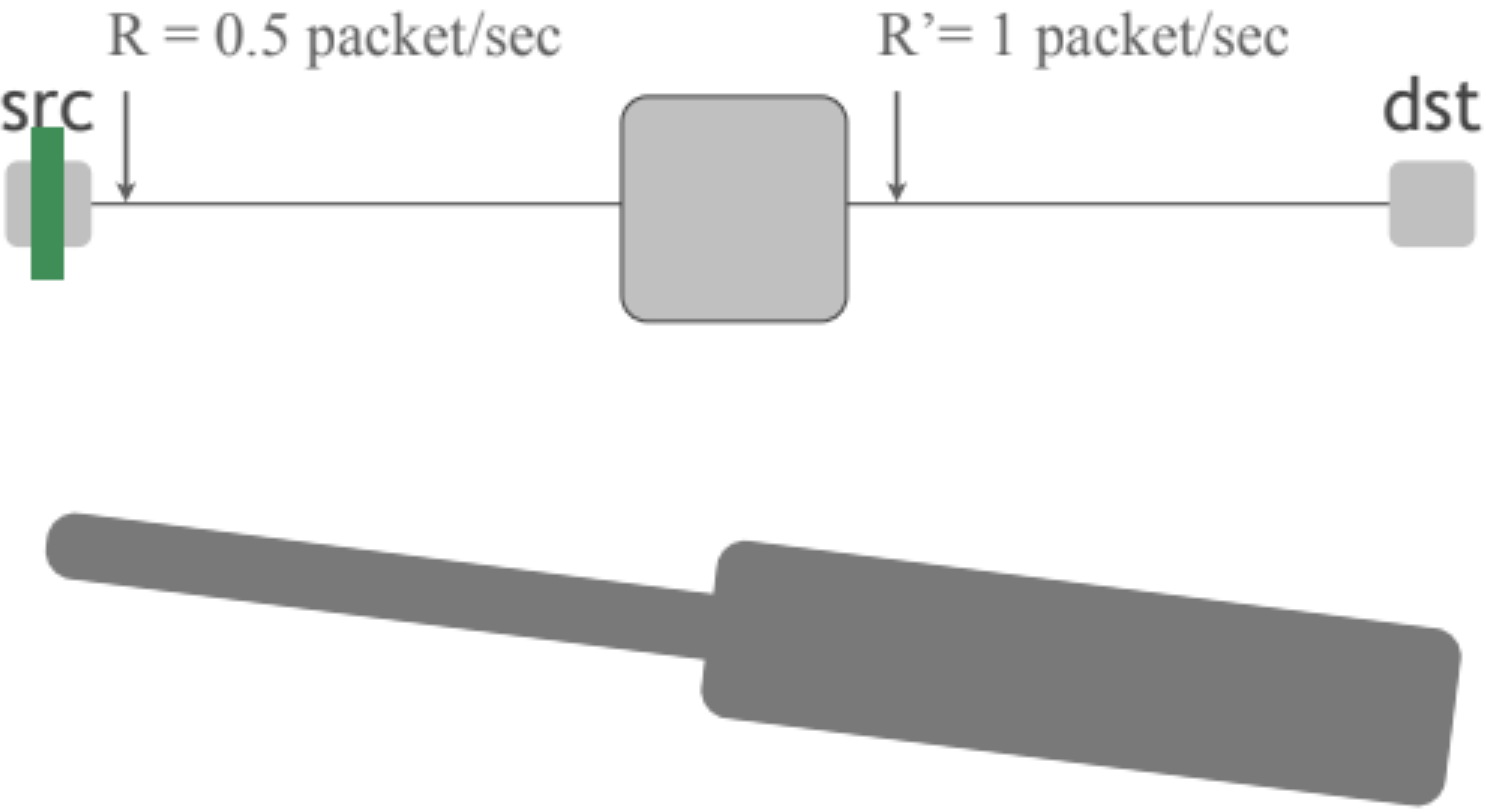
\includegraphics[width=.55\textwidth]{images/bottleneck_example2.png}
\end{center}
This resembles an inverted bottle where liquid enters through the narrow neck and exits through the wide opening. The bottleneck still determines the overall flow rate.

\subsubsection{Bottleneck Location}
When two end-systems communicate over the Internet, the bottleneck link is often at the edge of their communication path, near one of the end-systems. However, the bottleneck link is not always the one with the smallest transmission rate.

\begin{center}
  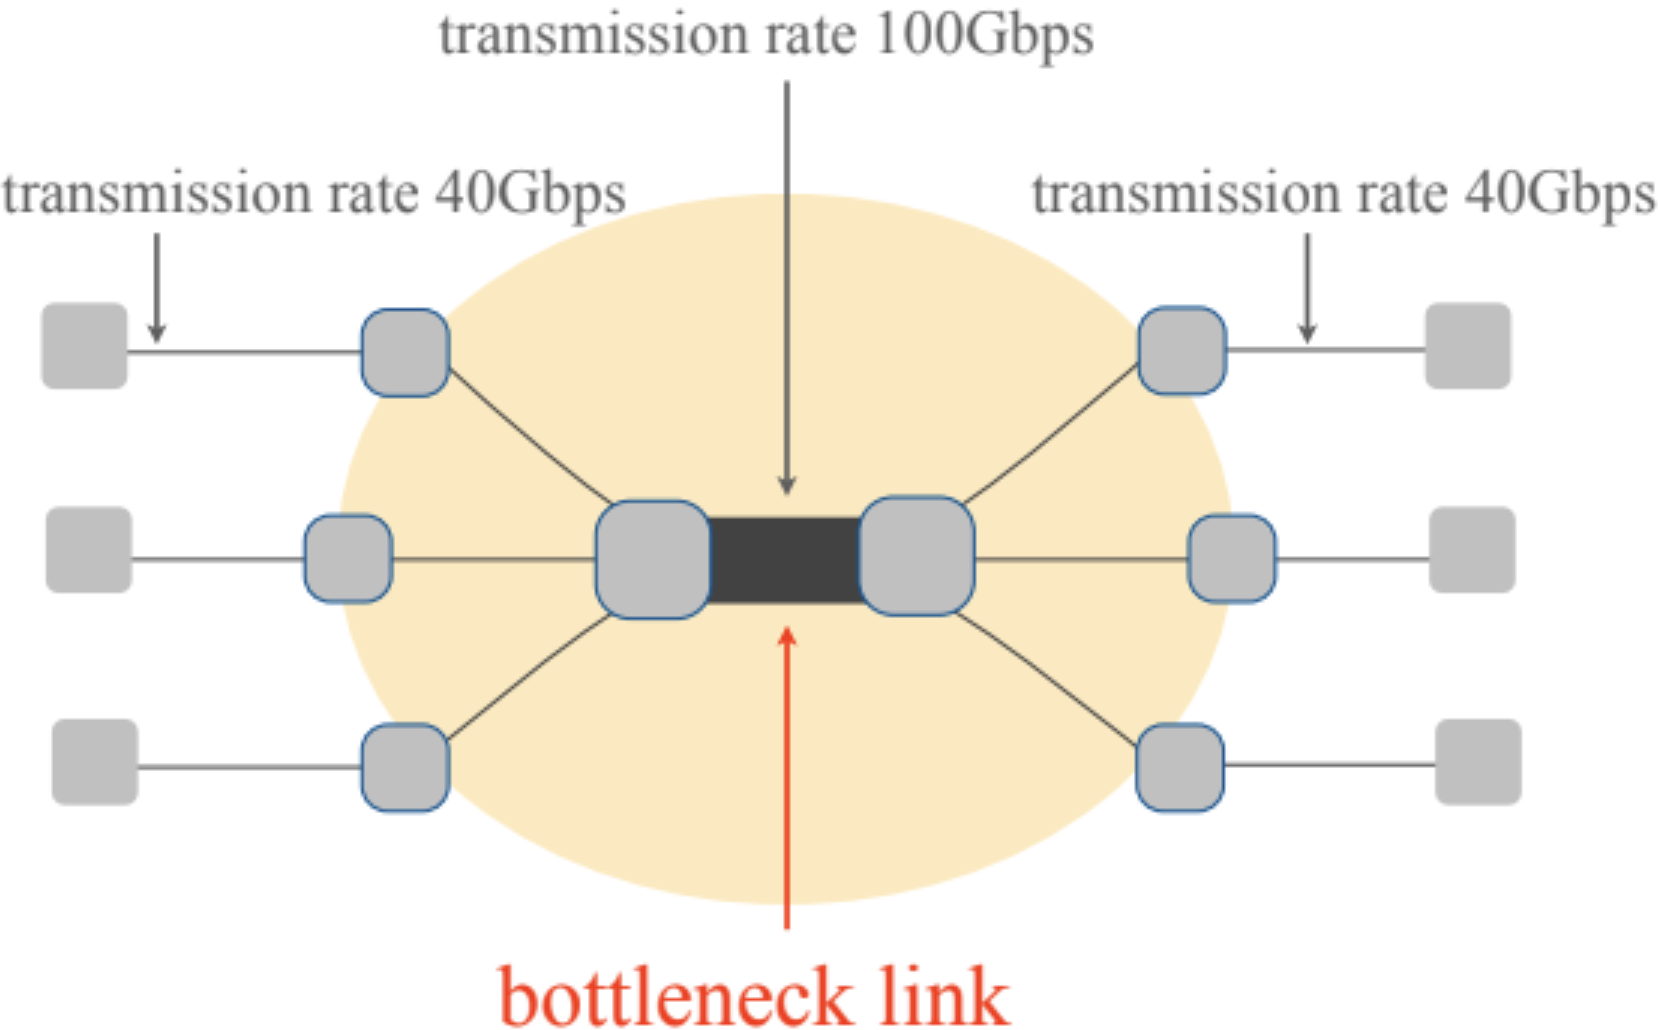
\includegraphics[width=.55\textwidth]{images/bottleneck.png}
\end{center}

\textbf{Example:} Consider a scenario where edge links have 40 Gbps transmission rates, while a middle link has 100 Gbps capacity. If the middle link receives aggregate traffic exceeding 100 Gbps from multiple sources, it becomes congested. The resulting queuing delay makes this high-capacity link the bottleneck, despite its superior transmission rate.

\section{Bottleneck Link Summary}
\textit{Key characteristics of bottleneck links.}

The bottleneck link between communicating end-systems is defined as the link where traffic flows at the slowest rate. This can occur due to two primary factors:

\begin{itemize}
  \item[-] \textbf{Low transmission rate} — the link has insufficient capacity
  \item[-] \textbf{Queuing delay} — the link becomes congested due to excessive traffic load
\end{itemize}

Understanding bottleneck identification and mitigation is crucial for network performance optimization and capacity planning.

\section{Resource Management in Packet Switches}
\textit{Understanding different approaches to managing network resources.}

To understand Internet performance characteristics, we must examine how packet switches manage their resources. There are two fundamental approaches to resource management in packet-switched networks.

\subsection{Packet Switching}
\textit{Resources allocated on-demand per packet.}

In packet switching, when a packet arrives at a switch, the switch decides whether it has sufficient resources (e.g., queue space) to store and process the packet. If resources are available, the switch uses its forwarding table to select the appropriate outgoing link and places the packet in the corresponding queue. Otherwise, the switch drops the packet.

Key characteristics:
\begin{itemize}
  \item[-] Each packet is treated as an independent entity
  \item[-] Resources are allocated on-demand
  \item[-] Admission and forwarding decisions are made per packet
\end{itemize}

\subsection{Circuit Switching}
\textit{Resources reserved in advance for virtual circuits.}

Circuit switching (specifically virtual circuit switching) creates the illusion of dedicated physical circuits without requiring actual dedicated links. When a source wants to communicate with a destination, it contacts all switches on the path and requests: "This source wants to communicate with this destination, sending at a maximum rate of $X$ Mbps, over the next $Y$ minutes. Can you accommodate this?"

\subsubsection{Virtual Circuit Establishment}
If a switch accepts the request, it:
\begin{enumerate}
  \item Chooses the best outgoing link for the destination
  \item Reserves the necessary capacity ($X$ Mbps) on that link
  \item Allocates a dedicated queue for the source/destination pair
  \item Commits to serving this queue at the requested rate
\end{enumerate}

If all switches on the path accept the request, a \textbf{virtual circuit} is established. As long as the source doesn't exceed $X$ Mbps, its packets experience no packet loss or unpredictable queuing delay.

Key characteristics:
\begin{itemize}
  \item[-] Traffic from each source/destination pair is treated as one entity
  \item[-] Resources are reserved in advance
  \item[-] Admission and forwarding decisions are made per virtual circuit
\end{itemize}

\subsection{Performance Comparison}
\textit{Analyzing the trade-offs between the two approaches.}

\subsubsection{Circuit Switching Analysis}

\paragraph{Advantages: Predictable Performance.} Consider a switch participating in two virtual circuits, both using the same 1 Gbps outgoing link. Each virtual circuit reserves 500 Mbps. As long as each circuit sends no more than its reserved rate, there is no packet loss or unpredictable queuing delay.

\paragraph{Disadvantages: Resource Inefficiency.} If one virtual circuit (e.g., orange) becomes silent while another (e.g., green) wants to send 1 Gbps, the switch cannot accommodate the green circuit's extra traffic. Reserved resources for the silent orange circuit remain unused, similar to a restaurant table reservation where the customer doesn't show up. This inefficiency occurs when the system turns down service requests despite having idle resources.

\subsubsection{Packet Switching Analysis}

\paragraph{Advantages: Resource Efficiency.} Without reservations, sources send packets into common queues per outgoing link. Whether two sources each send 500 Mbps simultaneously, or one source sends 1 Gbps while the other is silent, the system accommodates all traffic up to the link capacity. Packets are never dropped if the switch has available resources.

\paragraph{Disadvantages: Unpredictable Performance.} Consider a scenario where one source consumes all available switch resources at 1 Gbps. When a second source attempts to send packets, they will likely be dropped due to resource exhaustion. Unlike circuit switching, packet switching provides no performance guarantees.

\subsection{Implementation Complexity}
\textit{Comparing the complexity of each approach.}

Packet switching is simpler to implement, requiring no special mechanisms at switches. Circuit switching requires more sophisticated switches that can:
\begin{itemize}
  \item[-] Evaluate and accept/reject reservation requests
  \item[-] Determine appropriate resource allocations per request
  \item[-] Perform actual resource reservation and management
\end{itemize}

However, packet switching introduces its own complexity: the need for \textbf{congestion control}. Without congestion control, aggressive sources can monopolize switch resources, preventing other sources from sending packets effectively.

\subsection{Resource Management Summary}
\textit{Comparing the fundamental trade-offs.}

\begin{itemize}
  \item[-] \textbf{Packet switching:} Efficient resource use, no performance guarantees, simpler to implement but requires congestion control
  \item[-] \textbf{Circuit switching:} Performance guarantees, inefficient resource use, more complex to implement
\end{itemize}

The Internet uses packet switching, which is why it offers a \textbf{"best effort" service}. There is no guarantee that packets will be delivered. When traffic traverses multiple packet switches, each switch does its best to store and process packets without typically reserving resources in advance.

\section{Statistical Multiplexing}
\textit{Efficient resource sharing based on statistical behavior of users.}

Statistical multiplexing occurs when many users share the same resource, but not all users are expected to be active simultaneously. This principle enables packet switching to support significantly more users than circuit switching.

\subsection{Video Server Example}
\textit{Demonstrating the benefits of statistical multiplexing.}

Consider a video server connected to a switch via a 10 Gbps link. Video clients connect to the switch and download videos, requiring at least 1 Gbps each for reasonable performance. Each client downloads only 10\% of the time (the remainder is spent watching the downloaded content).

\subsubsection{Circuit Switching Capacity}
With circuit switching, the switch must reserve 1 Gbps for each client. Given the 10 Gbps link capacity, the switch can serve at most \textbf{10 clients}.

\subsubsection{Packet Switching Capacity}
With packet switching and the 10\% activity rate, the switch can serve approximately \textbf{35 clients}. The probability that 10 or fewer clients are downloading simultaneously is 99.96\%, providing nearly the same performance as circuit switching while serving more than three times as many clients.

\subsection{Resource Efficiency Example}
\textit{Illustrating dynamic resource allocation.}

Consider 10 potential clients where only one is active, downloading a 10 Gb video file:

\begin{itemize}
  \item[-] \textbf{Circuit switching:} With 1 Gbps reserved per client, the download takes 10 seconds
  \item[-] \textbf{Packet switching:} The active client can use the full 10 Gbps capacity, completing the download in 1 second
\end{itemize}

This demonstrates efficient resource utilization: inactive clients don't consume resources, allowing active clients to achieve better performance.

\subsection{Historical Context: Traditional Circuit Switching}
\textit{Understanding the origins of circuit switching terminology.}

Traditional telephone networks used actual circuit switches that created dedicated physical circuits. When a source wanted to communicate with a destination, a \textbf{circuit establishment phase} configured each circuit switch on the path to create a real physical circuit. Once established, the switches played no further role—the source could send signals directly to the destination through the dedicated physical circuit.

Modern "virtual" circuit switching simulates this behavior without requiring dedicated physical circuits, using resource reservations to provide similar guarantees.
\newpage
\section{Circuit Implementation Techniques}
\textit{Different approaches to creating circuit-switched communications.}

There are multiple ways to implement circuit switching, each creating the illusion of separate physical circuits for communicating pairs while sharing physical infrastructure.

\subsection{Types of Circuits}
\textit{Physical versus virtual circuit implementations.}

\begin{itemize}
  \item[-] \textbf{Physical circuits:} Separate sequence of physical links per communicating end-system pair
  \item[-] \textbf{Virtual circuits:} Manage resources as if there was a separate sequence of physical links per communicating pair
\end{itemize}

\subsection{Multiplexing Techniques}
\textit{Methods for sharing physical resources among multiple communications.}

\subsubsection{Time Division Multiplexing (TDM)}
A single physical circuit is divided into time slots, with each source/destination pair assigned a separate time slot. This is analogous to a classroom used by multiple courses, where each course uses the room during a different time period. Each class has the illusion of having their own classroom.

\subsubsection{Frequency Division Multiplexing (FDM)}
A single physical circuit's bandwidth is divided into frequency bands, with each source/destination pair assigned a separate frequency band. This resembles radio broadcasting, where multiple stations share the airwaves but each uses a different frequency band.

Both techniques create the illusion of dedicated physical circuits while efficiently sharing underlying physical resources.

\section{System Design Considerations}
\textit{Choosing between on-demand and reservation-based approaches.}

\subsection{The Restaurant Analogy}
\textit{Understanding the fundamental trade-offs through a familiar example.}

Consider designing a restaurant's reservation policy:

\paragraph{No Reservations (On-Demand):}
\begin{itemize}
  \item[-] Restaurant stays maximally utilized when customers keep arriving
  \item[-] Customers may wait or leave when capacity is exceeded
  \item[-] Higher resource efficiency but unpredictable service quality
\end{itemize}

\paragraph{Reservation System:}
\begin{itemize}
  \item[-] Tables must be held for reserved customers who may not show up
  \item[-] Guaranteed service for customers with reservations
  \item[-] Lower resource efficiency but predictable service quality
\end{itemize}

\subsection{Network Design Trade-offs}
\textit{Applying the restaurant analogy to network systems.}

The choice between packet switching (on-demand) and circuit switching (reservations) requires balancing:

\begin{itemize}
  \item[-] \textbf{Infrastructure cost and complexity} versus \textbf{quality of service guarantees}
  \item[-] \textbf{Resource utilization efficiency} versus \textbf{performance predictability}
  \item[-] \textbf{Implementation simplicity} versus \textbf{service reliability}
\end{itemize}

Network designers must evaluate these trade-offs based on application requirements, user expectations, and economic constraints to determine the most appropriate resource management approach.

\section{Network Security Considerations}
\textit{Understanding threats and vulnerabilities in shared networks.}

When multiple users share a network, there are opportunities for misbehavior. Network security must address various types of malicious activities that can compromise communication integrity, confidentiality, and availability.

\subsection{Common Network Threats}
\textit{Categorizing different types of network attacks.}

\subsubsection{Eavesdropping (Sniffing)}
\textbf{Eve the eavesdropper} attempts to listen in on communications between legitimate users (e.g., Alice and Bob) and copy their data. This passive attack compromises confidentiality by allowing unauthorized access to private information.

\subsubsection{Impersonation (Spoofing)}
\textbf{Persa the impersonator} pretends to be a legitimate user (e.g., Alice) to extract information from another user (e.g., Bob). Unlike eavesdropping, this is an active attack where the attacker generates traffic and participates in the communication.

\subsubsection{Denial of Service (DoS)}
\textbf{Denis the denial-of-service attacker} disrupts communication between legitimate users by consuming network or system resources. This can be accomplished by:
\begin{itemize}
  \item[-] Sending excessive junk traffic to exhaust the target's resources
  \item[-] Coordinating attacks using multiple compromised systems (\textbf{Distributed DoS})
  \item[-] Enlisting networks of compromised computers (\textbf{botnets})
\end{itemize}

\subsubsection{Malware}
\textbf{Malik the malware master} infects users' computers with malicious software designed to:
\begin{itemize}
  \item[-] Delete or corrupt data
  \item[-] Steal sensitive information
  \item[-] Force computers to send spam or participate in attacks
  \item[-] Provide unauthorized remote access to systems
\end{itemize}

\subsection{Trust Models in System Design}
\textit{Defining assumptions about user behavior.}

A critical design question for any computing/communication system is determining what to assume about user behavior. Trust models define the security assumptions and threat models that inform system design decisions.

\section{Fundamental Design Questions}
\textit{Key considerations for computing and communication systems.}

Through our examination of Internet architecture and performance, several fundamental questions emerge that must be addressed when designing any computing or communication system:

\begin{enumerate}
  \item \textbf{What physical infrastructure is already available?} — Understanding existing resources and constraints
  \item \textbf{What layers to define?} — Determining system architecture and abstraction boundaries
  \item \textbf{Treat on demand or take reservations?} — Choosing between dynamic allocation and advance reservation
  \item \textbf{What trust model to design for?} — Defining security assumptions and threat models
\end{enumerate}

These questions form the foundation for making informed architectural decisions that balance performance, security, complexity, and cost considerations in system design.

\end{document}
